% Prisoners' Dilemma
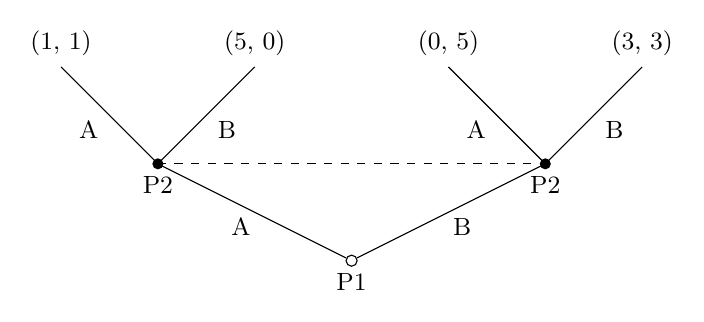
\begin{tikzpicture}[x=1pt, y=1pt, every node/.style={inner sep=1pt, font=\small}]
  \node[anchor=south] at (175,0) {P1};
  \draw (175,12) circle (2);
  \draw (173,13) -- (104,47.5);
  \draw (177,13) -- (246,47.5);
  \node[anchor=south] at (135,20) {A};
  \node[anchor=south] at (215,20) {B};
  \node[anchor=south] at (105,35) {P2};
  \fill (105,47) circle (2);
  \draw (105,47) -- (70,82);
  \node[anchor=south] at (70,85) {(1, 1)};
  \draw (105,47) -- (140,82);
  \node[anchor=south] at (140,85) {(5, 0)};
  \node[anchor=south] at (80,55) {A};
  \node[anchor=south] at (130,55) {B};
  \node[anchor=south] at (245,35) {P2};
  \fill (245,47) circle (2);
  \draw (245,47) -- (210,82);
  \node[anchor=south] at (210,85) {(0, 5)};
  \draw (245,47) -- (280,82);
  \node[anchor=south] at (280,85) {(3, 3)};
  \node[anchor=south] at (220,55) {A};
  \node[anchor=south] at (270,55) {B};
  \draw[dashed] (105,47) -- (243,47);
\end{tikzpicture}
